\begin{frame}{Path merged : thread 9}
    \setbeamercovered{invisible}
\RaggedRight
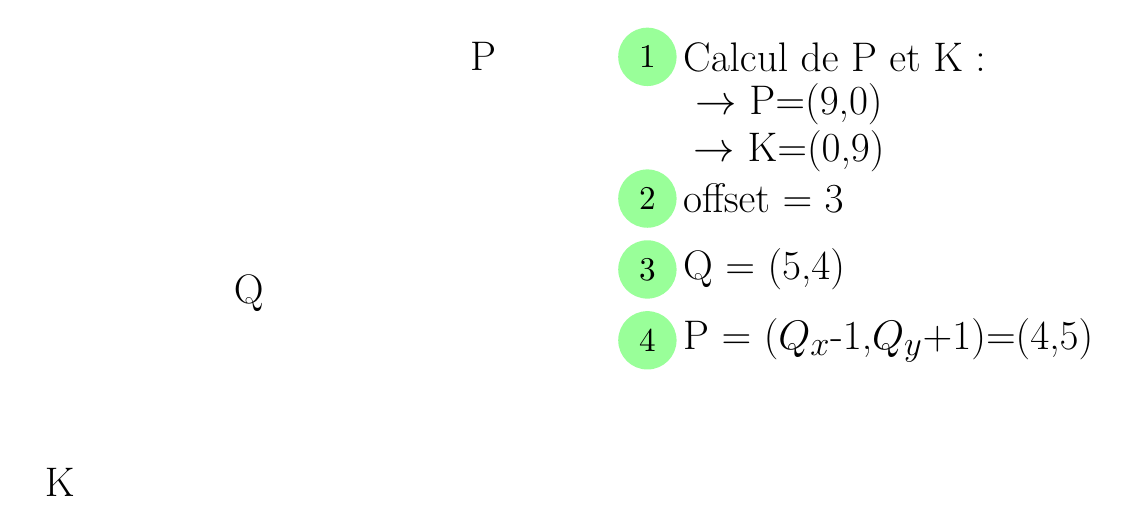
\begin{tikzpicture}[line cap=round,scale=0.6, every node/.style={transform shape}]
    \baseGraph
    \draw (-3,6) node {\BlueRoute}; 
    \maze (-3,6) node {\BlueRoute}--(-3,5)node {\BlueRoute};
    \maze (-3,5) node {\BlueRoute}--(-3,4)node {\BlueRoute};
    \maze (-3,4) node {\BlueRoute}--(-2,4)node {\BlueRoute};
    \maze (-2,4) node {\BlueRoute}--(-2,3)node {\BlueRoute};
    \maze (-2,3) node {\BlueRoute}--(-2,2)node {\BlueRoute};
    \maze (-2,2) node {\BlueRoute}--(-2,1)node {\BlueRoute};
    \maze (-2,1) node {\BlueRoute}--(-1,1) node {\BlueRoute};
    \maze (-1,1) node {\BlueRoute}--(0,1) node {\BlueRoute};
    \maze (0,1)  node {\BlueRoute}--(0,0) node {\BlueRoute}; %ajouter ce qu'on a déjà fait 
    \draw (10,6) node[shape = circle,label=right:\Huge{Calcul de P et K :},fill=green!40,scale=2] {1};\pause 
    \draw (13,5) node {\Huge{$\rightarrow$ P=(9,0)}}; 
    \draw (6,6) node[label=right:\Huge{P}] {\BlackCirc};\pause
    \draw (13,4) node {\Huge{$\rightarrow$ K=(0,9)}};
    \draw (-3,-3) node[label=right:\Huge{K}] {\BlackCirc};\pause
    \draw (10,3) node[shape = circle,label=right:\Huge{offset = 3},fill=green!40,scale=2] {2};\pause
    \draw (10,1.5) node[shape = circle,label=right:\Huge{Q = (5,4)},fill=green!40,scale=2] {3};
    \draw (1,1) node[label=right:\Huge{Q}] {\BlackCirc};\pause
    \draw (10,0) node[shape = circle,label=right:\Huge{P = ($Q_{x}$-1,$Q_{y}$+1)=(4,5)},fill=green!40,scale=2] {4};\pause 
    %\draw (10,-1.5) node[shape = circle,label=right:\Huge{M[i]=A[$Q_{y}$]},fill=green!40,scale=2] {5}; 
    %\draw (-3,6) node {\BlueRoute}; \pause
\end{tikzpicture}
\end{frame}


\begin{frame}{Path merged : thread 9}
    \setbeamercovered{invisible}
\RaggedRight
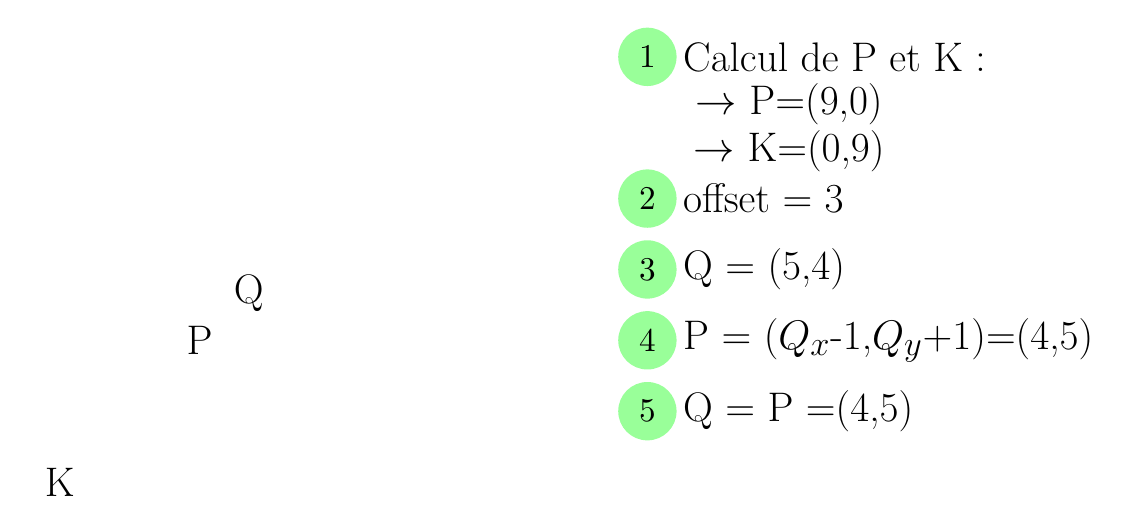
\begin{tikzpicture}[line cap=round,scale=0.6, every node/.style={transform shape}]
    \baseGraph
    \draw (-3,6) node {\BlueRoute}; 
    \maze (-3,6) node {\BlueRoute}--(-3,5)node {\BlueRoute};
    \maze (-3,5) node {\BlueRoute}--(-3,4)node {\BlueRoute};
    \maze (-3,4) node {\BlueRoute}--(-2,4)node {\BlueRoute};
    \maze (-2,4) node {\BlueRoute}--(-2,3)node {\BlueRoute};
    \maze (-2,3) node {\BlueRoute}--(-2,2)node {\BlueRoute};
    \maze (-2,2) node {\BlueRoute}--(-2,1)node {\BlueRoute};
    \maze (-2,1) node {\BlueRoute}--(-1,1) node {\BlueRoute};
    \maze (-1,1) node {\BlueRoute}--(0,1) node {\BlueRoute};
    \maze (0,1)  node {\BlueRoute}--(0,0) node {\BlueRoute}; %ajouter ce qu'on a déjà fait 
    \draw (10,6) node[shape = circle,label=right:\Huge{Calcul de P et K :},fill=green!40,scale=2] {1}; 
    \draw (13,5) node {\Huge{$\rightarrow$ P=(9,0)}}; 
    \draw (0,0) node[label=right:\Huge{P}] {\BlackCirc};
    \draw (13,4) node {\Huge{$\rightarrow$ K=(0,9)}};
    \draw (-3,-3) node[label=right:\Huge{K}] {\BlackCirc};
    \draw (10,3) node[shape = circle,label=right:\Huge{offset = 3},fill=green!40,scale=2] {2};
    \draw (10,1.5) node[shape = circle,label=right:\Huge{Q = (5,4)},fill=green!40,scale=2] {3};
    \draw (1,1) node[label=right:\Huge{Q}] {\BlackCirc};
    \draw (10,0) node[shape = circle,label=right:\Huge{P = ($Q_{x}$-1,$Q_{y}$+1)=(4,5)},fill=green!40,scale=2] {4}; 
    \draw (10,-1.5) node[shape = circle,label=right:\Huge{Q = P =(4,5)},fill=green!40,scale=2] {5}; 
    %\draw (10,-1.5) node[shape = circle,label=right:\Huge{M[i]=A[$Q_{y}$]},fill=green!40,scale=2] {5}; 
    %\draw (-3,6) node {\BlueRoute}; \pause
\end{tikzpicture}
\end{frame}

\begin{frame}{Path merged : thread 9}
    \setbeamercovered{invisible}
\RaggedRight
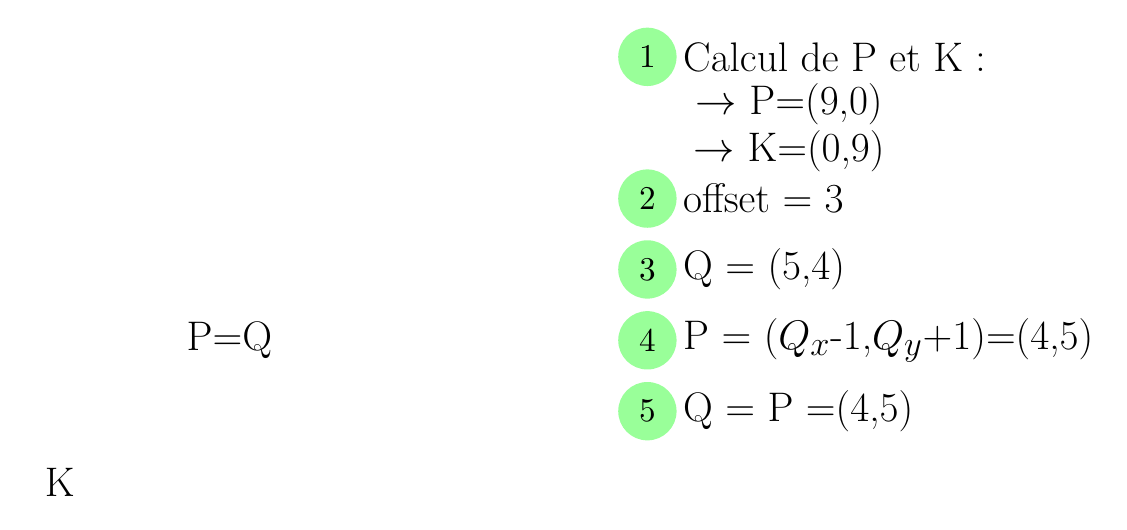
\begin{tikzpicture}[line cap=round,scale=0.6, every node/.style={transform shape}]
    \baseGraph
    \draw (-3,6) node {\BlueRoute}; 
    \maze (-3,6) node {\BlueRoute}--(-3,5)node {\BlueRoute};
    \maze (-3,5) node {\BlueRoute}--(-3,4)node {\BlueRoute};
    \maze (-3,4) node {\BlueRoute}--(-2,4)node {\BlueRoute};
    \maze (-2,4) node {\BlueRoute}--(-2,3)node {\BlueRoute};
    \maze (-2,3) node {\BlueRoute}--(-2,2)node {\BlueRoute};
    \maze (-2,2) node {\BlueRoute}--(-2,1)node {\BlueRoute};
    \maze (-2,1) node {\BlueRoute}--(-1,1) node {\BlueRoute};
    \maze (-1,1) node {\BlueRoute}--(0,1) node {\BlueRoute};
    \maze (0,1)  node {\BlueRoute}--(0,0) node {\BlueRoute}; %ajouter ce qu'on a déjà fait 
    \draw (10,6) node[shape = circle,label=right:\Huge{Calcul de P et K :},fill=green!40,scale=2] {1}; 
    \draw (13,5) node {\Huge{$\rightarrow$ P=(9,0)}}; 
    \draw (13,4) node {\Huge{$\rightarrow$ K=(0,9)}};
    \draw (-3,-3) node[label=right:\Huge{K}] {\BlackCirc};
    \draw (10,3) node[shape = circle,label=right:\Huge{offset = 3},fill=green!40,scale=2] {2};
    \draw (10,1.5) node[shape = circle,label=right:\Huge{Q = (5,4)},fill=green!40,scale=2] {3};
    \draw (0,0) node[label=right:\Huge{P=Q}] {\BlackCirc};
    \draw (10,0) node[shape = circle,label=right:\Huge{P = ($Q_{x}$-1,$Q_{y}$+1)=(4,5)},fill=green!40,scale=2] {4}; 
    \draw (10,-1.5) node[shape = circle,label=right:\Huge{Q = P =(4,5)},fill=green!40,scale=2] {5}; 
    %\draw (10,-1.5) node[shape = circle,label=right:\Huge{M[i]=A[$Q_{y}$]},fill=green!40,scale=2] {5}; 
    %\draw (-3,6) node {\BlueRoute}; \pause
\end{tikzpicture}
\end{frame}

\begin{frame}{Path merged : thread 9}
    \setbeamercovered{invisible}
\RaggedRight
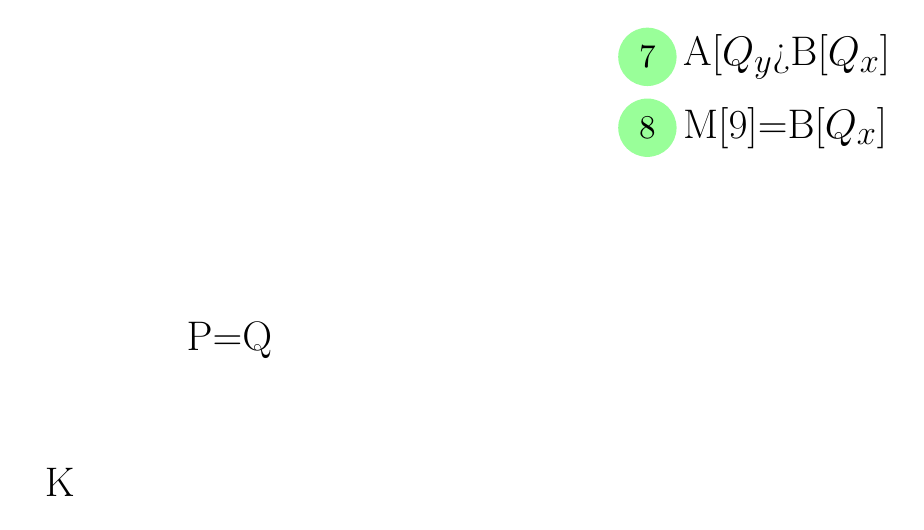
\begin{tikzpicture}[line cap=round,scale=0.6, every node/.style={transform shape}]
    \baseGraph
    \draw (-3,6) node {\BlueRoute}; 
    \maze (-3,6) node {\BlueRoute}--(-3,5)node {\BlueRoute};
    \maze (-3,5) node {\BlueRoute}--(-3,4)node {\BlueRoute};
    \maze (-3,4) node {\BlueRoute}--(-2,4)node {\BlueRoute};
    \maze (-2,4) node {\BlueRoute}--(-2,3)node {\BlueRoute};
    \maze (-2,3) node {\BlueRoute}--(-2,2)node {\BlueRoute};
    \maze (-2,2) node {\BlueRoute}--(-2,1)node {\BlueRoute};
    \maze (-2,1) node {\BlueRoute}--(-1,1) node {\BlueRoute};
    \maze (-1,1) node {\BlueRoute}--(0,1) node {\BlueRoute};
    \maze (0,1)  node {\BlueRoute}--(0,0) node {\BlueRoute}; %ajouter ce qu'on a déjà fait 
    \draw (-3,-3) node[label=right:\Huge{K}] {\BlackCirc};
    \draw (0,0) node[label=right:\Huge{P=Q}] {\BlackCirc};
    \draw (10,6) node[shape = circle,label=right:\Huge{A[$Q_{y}$>B[$Q_{x}$]},fill=green!40,scale=2] {7}; \pause
    \draw (10,4.5) node[shape = circle,label=right:\Huge{M[9]=B[$Q_{x}$]},fill=green!40,scale=2] {8};\pause
\end{tikzpicture}
\end{frame}


\begin{frame}{Path merged : thread 9, path}
    \setbeamercovered{invisible}
\RaggedRight
\begin{tikzpicture}[line cap=round,scale=0.6, every node/.style={transform shape}]
    \baseGraph
    \draw (-3,6) node {\BlueRoute}; 
    \maze (-3,6) node {\BlueRoute}--(-3,5)node {\BlueRoute};
    \maze (-3,5) node {\BlueRoute}--(-3,4)node {\BlueRoute};
    \maze (-3,4) node {\BlueRoute}--(-2,4)node {\BlueRoute};
    \maze (-2,4) node {\BlueRoute}--(-2,3)node {\BlueRoute};
    \maze (-2,3) node {\BlueRoute}--(-2,2)node {\BlueRoute};
    \maze (-2,2) node {\BlueRoute}--(-2,1)node {\BlueRoute};
    \maze (-2,1) node {\BlueRoute}--(-1,1) node {\BlueRoute};
    \maze (-1,1) node {\BlueRoute}--(0,1) node {\BlueRoute};
    \maze (0,1)  node {\BlueRoute}--(0,0) node {\BlueRoute};
    \maze (0,0)  node {\BlueRoute}--(1,0) node {\BlueRoute};\pause
    \maze (1,0)  node {\BlueRoute}--(1,-1)node {\BlueRoute};\pause
    \maze (1,-1) node {\BlueRoute}--(4,-1)node {\BlueRoute};\pause
    \maze (4,-1) node {\BlueRoute}--(4,-2)node {\BlueRoute};\pause
    \maze (4,-2) node {\BlueRoute}--(4,-3)node {\BlueRoute};\pause
    
\end{tikzpicture}
\end{frame}